\section{Wurzelkörper und Zerfällungskörper}
Sei $K$ ein Körper, $f \in K[X]$ mit $n = \deg(f) > 0$.
\begin{example}
	Sei $K=\Q$. Dann hat $f$ eine Nullstelle (``Wurzel'') $\alpha \in \C$, und $L:= K(\alpha) = K[\alpha]$ ist die kleinste Erweiterung von $\Q$ in $\C$, die diese Nullstelle enthält.
\end{example}
\begin{definition}[Wurzelkörper]
	Ein \begriff{Wurzelkörper} von $f$ ist eine Körpererweiterung $L \mid K$ der Form $L = K(\alpha)$ mit $f(\alpha) = 0$.
\end{definition}
\begin{lemma}
	\proplbl{1_3_3}
	Sei $L = K(\alpha)$ mit $f(\alpha) = 0$ ein Wurzelkörper von $f$. Dann ist $[L:K] \le n$. Ist $f$ irreduzibel, so ist $[L:K] = n$ und $g \mapsto g(\alpha)$ induziert einen Isomorphismus $\lnkset{K[X]}{(f)} \overset{\cong}{\longrightarrow}_K L$.
\end{lemma}
\begin{proof} %TODO fix b) ref
	Sei zunächst $f$ irreduzibel, $f_{\alpha} = \MinPol(\alpha \mid K)$. Dann ist $f = cf_{\alpha}$, die Behauptung folgt somit aus \propref{1_2_7}b). Für $f \in K[X]$ beliebig, schreibe $f = f_1\cdots f_r$ mit $f_i \in K[X]$ irreduzibel
	\begin{align*}
		f(\alpha) = 0 \Rightarrow \text{ OE } f_1(\alpha) = 0 \Rightarrow [L:K] = \deg(f_1) \le \deg(f) = n %TODO is it really 1 in the index?
	\end{align*}
\end{proof}
\begin{lemma}
	\proplbl{1_3_4}
	Sei $f$ irreduzibel. Dann ist $L := \lnkset{K[X]}{(f)}$ ein Wurzelkörper von $f$.
\end{lemma}
\begin{proof}
	Betrachte den Epimorphismus $\pi = \pi_f: K[X] \to \lnkset{K[X]}{(f)} = L$, setze $\alpha = \pi(X)$
	\begin{itemize}
		\item $K$ Körper $\Rightarrow \pi_{\mid K}$ injektiv\\
		$\Rightarrow$ können $K$ mit Teilkörper von $L$ identifizieren, sodass $\pi_{\mid K} = \id_K$
		\item $(f)$ irreduzibel $\Rightarrow$ prim $\xrightarrow{\text{GEO II.4.7}}$ $(f)$ maximal $\Rightarrow L = \lnkset{K[X]}{(f)}$ ist Körper
		\item $f(\alpha) = f(\pi(X)) \overset{(\ast)}{=} \pi(f(X)) = 0 \quad f(X) \in \Ker(\pi)$\\
		($\ast$ gilt, da $f = \sum a_i x^i = \pi(f) = \sum \pi(a_i)\pi(x)^i = \sum a_i \pi(x)^i = f(\pi(x))$)
		\item $L=\pi(K[X]) = K[\pi(X)] = k[\alpha] \overset{\alpha \text{ alg.}}{=} K(\alpha)$
	\end{itemize}
\end{proof}
\begin{proposition}
	\proplbl{1_3_5}
	Sei $f$ irreduzibel. Ein Wurzelkörper von $f$ existiert und ist eindeutig in folgendem Sinn:\\
	Sind $L_1 = K(\alpha_1), L_2 = K(\alpha_2)$ mit $f(\alpha_1) = 0 = f(\alpha_2)$, so existiert genau ein $K$-Isomorphismus $\varphi: L_1 \to L_2$ mit $\varphi(\alpha_1) = \alpha_2$.
\end{proposition}
\begin{proof}\
	\begin{itemize}
		\item Existenz gibt \propref{1_3_4}
		\item \propref{1_3_3} liefert Isomorphismus
		\begin{align*}
			\begin{Bmatrix} %TODO find a way to only have the right curly bracket!
				L_1 \xleftarrow[\varphi_1]{\cong} & \lnkset{K[X]}{(f)} & \xrightarrow[\varphi_2]{\cong} L_2\\
				\alpha_1 \mapsfrom & X + (f) & \mapsto \alpha_2\\
			\end{Bmatrix}
			\Rightarrow \varphi_2 \circ \varphi_1 : L_1 \xrightarrow{\cong}_K L_2 \mit \alpha_1 \mapsto \alpha_2
		\end{align*}
		Umgekehrt ist jeder $K$-Isomorphismus $\varphi: L_1 \to_K L_2$ wegen $L_1 = K(\alpha_1)$ schon durch $\varphi(\alpha_1)$ festgelegt.
	\end{itemize}
\end{proof}
\begin{conclusion}
	\proplbl{1_3_6}
	$f$ hat einen Wurzelkörper.
\end{conclusion}
\begin{proof}
	Schreibe $f=f_1\cdots f_r, f_1,\dots,f_r \in K[X]$ irreduzibel, nehme einen Wurzelkörper von $f_1$.
\end{proof}
\begin{conclusion}
	\proplbl{1_3_7}
	Es gibt eine Erweiterung $L\mid K$, über der $f$ in Linearfaktoren zerfällt, also $f=c\prod_{i=0}^{n}(x-\alpha_i)$ mit $c \in K^{\times}, \alpha,\dots,\alpha_n \in L$. 
\end{conclusion}
\begin{proof}
	Schreibe $f=c\cdot f_0 \mit c \in K^{\times}, f_0 \in K[X]$ normiert.\\ Induktion nach $n$:
	\begin{itemize}
		\item $n=1:$ $f = x-a$, nehme $L=K$.
		\item $n>1:$ Nach \propref{1_3_6} existiert $L_1 \mid K, \alpha_1 \in L_1 \mit f_0 (\alpha_1) = 0$\\
		$\Rightarrow$ $f_0 = (x-\alpha_1)\cdot f_1 \mit f_1 \in L_1 [X]$ normiert\\
		$\xRightarrow{\text{(IH)}}$ existiert $L\mid L_1 , \alpha_1, \dots, \alpha_n \in L \mit f_1 = \prod_{i=2}^n (x - \alpha_i)$\\
		$\Rightarrow$ $f = c\cdot f_0 = c\cdot (x-\alpha_1) \cdot f_1 = c \prod_{i=1}^n (x- \alpha_i)$
	\end{itemize}
\end{proof}
\begin{definition}[Zerfällungskörper]
	Ein \begriff{Zerfällungskörper} von $K$ ist eine Erweiterung $L\mid K$ der Form $L = K(\alpha_1,\dots,\alpha_n)$ mit $f=c\mal \prod_{i=1}^n (x-\alpha_i) \mit c \in K^{\times}$.
\end{definition}
\begin{proposition}
	\proplbl{1_3_9}
	Ein Zerfällungskörper von $f$ existiert.
\end{proposition}
\begin{proof}
	Ist $L\mid K$ wie in \propref{1_3_7}, ist $K(\alpha_1,\dots,\alpha_n)$ ein Zerfällungskörper von $f$.
\end{proof}
\begin{lemma}
	Ist $L \mid K$ ein Zerfällungskörper vpn $f$, so ist $[L:K] \le n$!
\end{lemma}
\begin{proof}
	Sei $L = K(\alpha_1,\dots,\alpha_n), f = c\prod_{i=1}^n (x-\alpha_i)$.\\
	Induktion nach $n$:
	\begin{itemize}
		\item $n=1:$ $L=K, [K:K] = 1$
		\item $n>1:$ $L_1 = K(\alpha_1)$ ist Wurzelkörper von $f \xRightarrow{\propref{1_3_3}} [L_1:K] \le n$ und schreibe $f=c\mal (x-\alpha_1)\mal f_1, f_1 = \prod_{i=2}^n (x-\alpha_i) \in L_1[X]$\\
		$\Rightarrow L = K(\alpha_1,\dots,\alpha_n) = L_1(\alpha_1,\dots,\alpha_n)$ ist Zerfällungskörper von $f_1$ (über $L_1$)\\
		$\xRightarrow{\text{IH}} [L:L_1] \le \deg(f_1)! = (n-1)!$\\
		$\Rightarrow [L:K] = [L:L_1][L_1:K] = (n-1)!n = n!$
	\end{itemize}
\end{proof}
\begin{example}
	\begin{enumerate}[label=(\alph*)]
		\item Ist $n=2$, so ist jeder Wurzelkörper $L$ von $f$, schon ein Zerfällungskörper: $[L:K]\le 2$.
		\item Ist $n =3$, $f$ irreduzibel. Schreibe $L_1 = K(\alpha), f = c(x-\alpha_1)f_1 \mit f_1 \in L_1[X]$
			\begin{itemize}
				\item $f_1$ reduzibel: $L_1$ ist schon Zerfällungskörper von $f$, $[L_1:K] = 3$
				\item $f_1$ irreduzibel: $L_1$ ist kein Zerfällungskörper von $f$. Ist $L$ Wurzelkörper von $f_1$, so ist $L$ Zerfällungskörper von $f$, $[L:K] = 3! = 6$
			\end{itemize}
	\end{enumerate}
\end{example}
\begin{*example}
	Sei $f = x^3 -2 \in \Q[X]$, dann sind die Nullstellen von $f$: $\sqrt[2]{2} \in \R, \zeta_3\sqrt[2]{2}, \zeta_3^2 \sqrt[2]{2}$
	\begin{itemize}
		\item $\Q(\sqrt[2]{2})$ ist Wurzelkörper von $f$. $\Q(\sqrt[3]{2}) \subseteq \R, \zeta_3\sqrt[3]{2}, \zeta_3^2 \sqrt[3]{2} \notin \R$, aber kein Zerfällungskörper. Der Zerfällungskörper von $f$ ist
		\begin{align*}
			\Q(\sqrt[3]{2},\zeta_3\sqrt[3]{2}, \zeta_3^2 \sqrt[3]{2}) = \Q(\sqrt[3]{2}, \zeta_3^2 \sqrt[3]{2})
		\end{align*}
	\end{itemize}
\end{*example}
\begin{mathematica}
	Will man die Nullstellen von $f = X^3 - 2 \in \Q[X]$ finden, dann bietet Mathematica folgende Funktion:
	\begin{align*}
		\texttt{Solve[f==0,x,Complexes]},
	\end{align*}
	der letzte Parameter lässt einem den Körper wählen, in dem Mathematica suchen soll. Es gibt zur Auswahl \texttt{Integers, Rationals, Reals, Complexes}. Für das Beispiel erhält man folgenden Output:
	\begin{align*}
		\set{x \to -(-2)^{(1/3)}, x \to 2^{(1/3)}, x \to (-1)^{(2/3)} 2^{(1/3)}}.
	\end{align*}
	Dabei müsste man die Einheitswurzeln identifizieren:
	\begin{align*}
		\set{x \to \zeta_3\sqrt[3]{2}, x \to \sqrt[3]{2}, x \to \zeta_3^2 \sqrt[3]{2}}
	\end{align*}
\end{mathematica}
\begin{*anmerkung}
	Wenn $f$ irreduzibel $\Rightarrow \lnkset{K[X]}{(f)}$ ist Wurzelkörper.
\end{*anmerkung}
\begin{lemma}
	\proplbl{1_3_12}
	Sei $f = \sum_{i=0}^n a_i x^i$ irreduzibel und sei $L = K(\alpha)$ mit $f(\alpha)$ ein Wurzelkörper von $f$. Sei $\tilde{L}\mid \tilde{K}$ eine weitere Körpererweiterung und $\varphi \in \Hom(K,\tilde{K})$. Ist $\sigma \in \Hom(L,\tilde{L})$ eine Fortsetzung von $\varphi$ (d.h. $\sigma_{\mid K} = \varphi$), so ist $\sigma(\alpha)$ eine Nullstelle von $f^{\varphi}=\sum_{i=0}^n \varphi(\alpha_i)x^i \in K[X]$. Ist umgekehrt $\beta \in L' $ eine Nullstelle von $f^{\varphi}$, so gibt es genau eine Fortsetzung $\sigma \in \Hom(L,\tilde{L})$ von $\varphi$ mit $\sigma(\alpha) = \beta$.
\begin{center} % tikzcd was bitchy, compiled and included the pdf.
	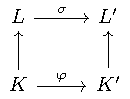
\includegraphics{./tikz/lemma_1_3_12.pdf}
\end{center}
\end{lemma}
\begin{proof}[was für die Prüfung!]
	\begin{itemize}
		\item $f(\alpha) = 0 \Rightarrow 0 = \sigma(0) = \sigma(f(\alpha)) = \sigma\brackets{\sum_{i=0}^n a_i \alpha_i} = \sum_{i=0}^n \varphi(a_i)\sigma(\alpha)^i = f^{\varphi}(\sigma(\alpha))$
		\item Eindeutigkeit klar, da $L=K(\alpha)$
		\item Existenz: Betrachte 
		\begin{align*}
			\eta: 
			\begin{cases}
				K[X] &\to L\\
				g &\mapsto g(\alpha)
			\end{cases}\qquad
			\psi:
			\begin{cases}
				K[X] &\to L'\\
				g &\to g^{\varphi}(\beta) 
			\end{cases}\qquad \to \text{ sind Homomorphismen nach univer. Eigenschaft}
		\end{align*}
		(Bemerke: $\eta$ surjektiv: $\eta_{\mid K} = \id \to K \in \Image(\eta) \mit \eta(x) = \alpha \to \alpha \in \Image(\eta)$)\\
		$Ker(\eta)=(f)$ ist Isomorphismus und $\bar{\eta}: \lnkset{K[X]}{(f)} \xrightarrow{\cong}L$ und\\
		$f \in \Ker(\psi) \Rightarrow \Ker(\psi) = (f)$ ist Homomorphismus $\bar{\psi}: \lnkset{K[X]}{(f)} \to L'$\\
		$\sigma:= \bar{\psi}\circ \bar{\eta}^{-1}: L \to L'$ ist eine Fortsetzung von $\psi$ und
		\begin{align*}
			\sigma(\alpha) = \bar{\psi}(x+(f)) = \beta
		\end{align*}
	\end{itemize}
\end{proof}
\begin{proposition}
	\proplbl{1_3_13}
	Der Zerfällungskörper von $f$ ist eindeutig bestimmt bis auf $K$-Isomorphie.
\end{proposition}
\begin{proof}
	\begin{enumerate}[label=]
		\item Behauptung: Ist $\varphi:K \to K'$ ein Isomorphismus, $L$ ein Zerfällungskörper, $L'$ ein Zerfällungs-körper von $f^{\varphi}$, so setzt sich $\varphi$ zu einem Isomorphismus $L \to L'$ fort.
		\item Beweis: Induktion nach $n = \deg(f)$
			\begin{enumerate}[label=] %TODO maybe use enum here without label?
				\item (IA) $n=1:$ $L = K \xrightarrow[\varphi]{\cong} K' = L'$ \checkmark
				\item (IS) $n>1:$ Schreibe $f = cg_1\cdots g_r$ mit $g_i \in K[x]$ normiert und irreduzibel, $c \in K^{\times}$\\
				$\Rightarrow f^{\varphi} = c^{\varphi}g_1^{\varphi}\cdots g_r^{\varphi}$ mit $c^{\varphi}\in (K')^{\varphi}$ und $g_i^{\varphi}\in K' [X]$ normiert und irreduzibel (weil $\varphi$ Isomorphismus ist). Sei $\alpha_1 \in L$ mit $g_1 (\alpha_1) = 0, \alpha'_1 \in L'$ mit $g_1^{\varphi}(\alpha'_1) = 0$\\
				$\xRightarrow{\propref{1_3_12}} \varphi$ setzt man zu einem Isomorphismus
				\begin{align*}
					\sigma: K_1 := K(\alpha_1) \to K' (\alpha'_1) \mit \sigma(\alpha_1) = \alpha'_1
				\end{align*} 
				fort. Schreibe $f=(x - \alpha_1)\cdot f_1^{\sigma}$ mit $f_1 \in K_1 [X]$ \\
				$\Rightarrow f^{\varphi} = (x - \underbrace{\sigma(\alpha_1)} _{\alpha'_1})\cdot f_1^{\sigma}$ mit $f_1^{\sigma}\in K'_1 [X]$. $L$ ist Zerfällungskörper von $f_1,L'$ ist Zerfällungskörper von $f_1^{\sigma}$\\
				$\Rightarrow \sigma$ setzt sich fort zu einem Isomorphismus $L \to L'$
			\end{enumerate}
		Die Behauptung im Fall $\varphi = \id_K$ ist genau die Aussage von \propref{1_3_13}.
	\end{enumerate}
\end{proof}
\begin{remark}
	Ist $M\mid K$ eine Erweiterung, die einem Zerfällungskörper $l$ von $f$ enthält, dann ist dieser nicht nur bis auf die Isomorphie sondern als Teilkörper eindeutig bestimmt $L = K(\alpha_1, \dots, \alpha_n)$, wobei $\alpha_1, \dots, \alpha_n$ genau die $n$ Nullstellen von $f$ in $M$ sind.
\end{remark}